\chapter{Planificación y metodología de trabajo}\label{cap:metodologia}

Este capítulo describe cómo se ha organizado el trabajo. Empieza por los objetivos de
gestión y por el método de desarrollo iterativo. Después detalla la metodología de ingeniería
gobernada mediante GSD, que el planteamiento del trabajo pide tratar como una aportación
observable y no como una nota al margen. Termina con la estimación de esfuerzo, los riesgos,
las lecciones de ingeniería más relevantes y las convenciones de commits y de idioma.

\section{Objetivos de gestión}\label{sec:met-objetivos-gestion}

La gestión del proyecto persigue cuatro objetivos. El primero es entregar valor de forma
incremental, con cada incremento vertical utilizable y verificado, en lugar de una
integración final de riesgo. El segundo es que toda afirmación de la memoria tenga respaldo:
una decisión registrada, una verificación independiente o una firma de aceptación. El tercero es
mantener el alcance bajo control a lo largo de sucesivos incrementos, sin que el trabajo de
uno contamine el de otro. El cuarto es que el proceso de ingeniería quede documentado con el
mismo rigor que el producto, de modo que un tercero pueda reconstruir no solo el sistema,
sino la secuencia de decisiones que lo produjo.

\section{Método de desarrollo iterativo}\label{sec:met-fases}

El ciclo de vida del proyecto se gobernó mediante el método \textit{Get Stuff Done}
(GSD)~\cite{gsd}, un sistema de desarrollo dirigido por especificación pensado para agentes de
código, versionado en el propio repositorio. GSD descompone el trabajo en incrementos
verticales y somete cada uno a un ciclo ordenado de cuatro pasos que la
Figura~\ref{fig:ciclo-gsd} resume: discutir, planificar, ejecutar y verificar. Cada paso
produce un artefacto escrito que actúa como fuente de verdad del siguiente. Lo que sobrevive
a los límites de sesión es la especificación escrita, no el historial de la conversación con
el agente.

\begin{figure}[H]
    \centering
    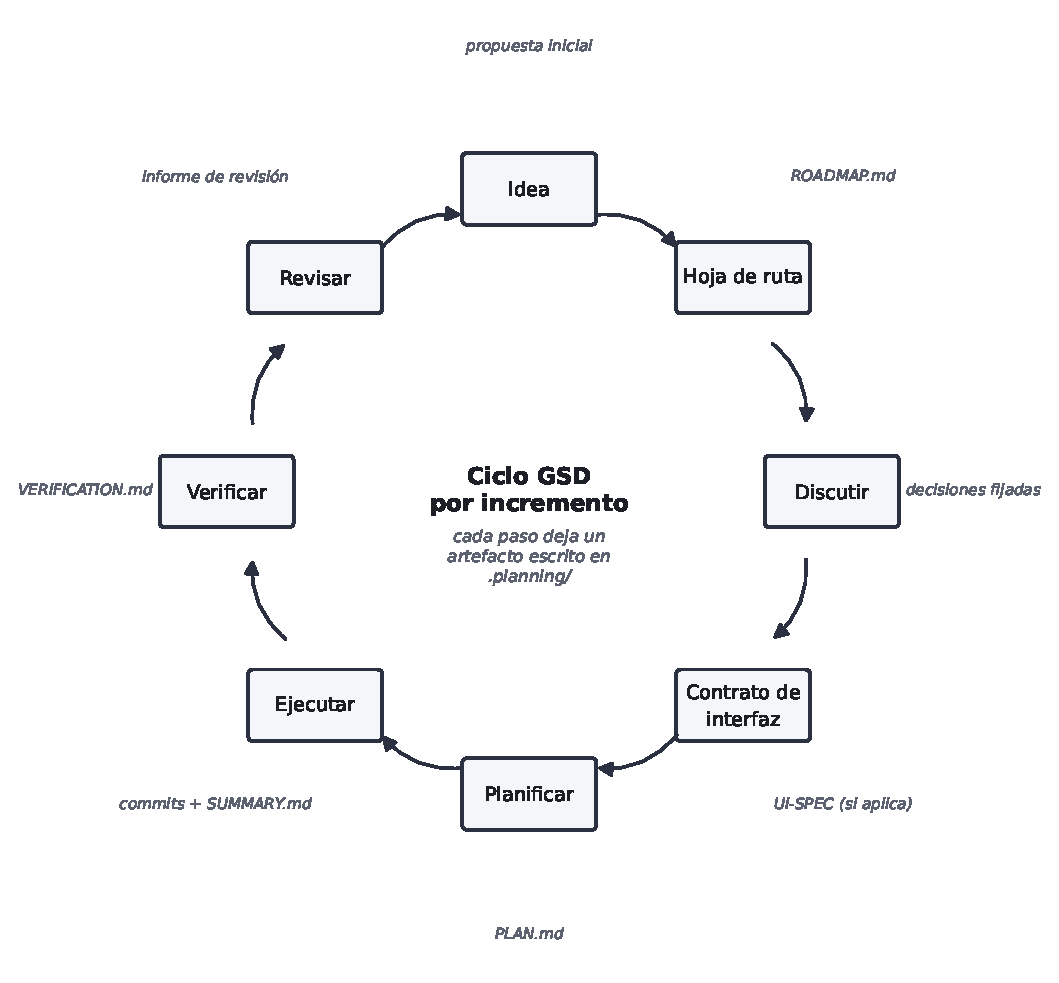
\includegraphics[width=0.72\textwidth]{figures/ciclo-gsd.pdf}
    \caption{Ciclo de un incremento en el método GSD y los artefactos que produce cada paso.}
    \label{fig:ciclo-gsd}
\end{figure}

En la práctica, cada incremento se abre con una discusión que fija por escrito sus decisiones
y supuestos. Si tiene interfaz, se establece además un contrato de diseño con sus componentes
y estados. A continuación se investiga y se redacta el plan, que lo descompone en tareas
atómicas con criterios de aceptación y se comprueba antes de tocar código. La ejecución
implementa ese plan, confirma los cambios en el control de versiones y registra en un resumen
lo realmente hecho y las desviaciones. Por último, la verificación comprueba, de forma
independiente, que el objetivo se ha alcanzado. Una revisión de código somete después los
cambios a un análisis de seguridad, rendimiento y corrección con un contexto distinto del que
los escribió. Cada incremento termina con una firma de aceptación del proyecto.

Las órdenes de este flujo se usaron de verdad durante el proyecto: \texttt{discuss-phase},
\texttt{ui-phase}, \texttt{plan-phase}, \texttt{execute-phase}, \texttt{verify-work},
\texttt{code-review}, además de \texttt{pause-work} y \texttt{resume-work} para suspender y
retomar el trabajo entre sesiones sin perder el hilo.

\section{Planificación viva: el árbol \texttt{.planning/}}\label{sec:met-planning}

GSD sustituye los documentos de planificación estáticos por un árbol de ficheros en formato
Markdown, versionados, que evolucionan con el proyecto. En \texttt{.planning/} conviven la
definición del producto (\texttt{PROJECT.md}), los requisitos operativos
(\texttt{REQUIREMENTS.md}), la hoja de ruta (\texttt{ROADMAP.md}) y una instantánea
del estado actual (\texttt{STATE.md}) que cualquier agente o persona lee antes de actuar.
Cada incremento se descompone en \texttt{.planning/phases/} en pares de plan y resumen: el
plan fija el alcance y los criterios de aceptación antes de implementar, mientras que el
resumen registra lo ejecutado, las desviaciones y las evidencias al cerrar. Junto a ellos
viven los documentos de contexto, investigación, contrato de interfaz, verificación e ítems
diferidos de cada incremento. Junto a este árbol normativo, el proyecto mantiene en
\texttt{ideas-vault/} un vault de Obsidian que enlaza los mismos conceptos entre sí de forma
navegable; el Capítulo~\ref{cap:gestion} lo describe con su propio grafo.

La Tabla~\ref{tab:planning-arbol} enumera los artefactos principales del árbol y su función.

\begin{table}[H]
\centering
\begin{tabularx}{\textwidth}{ | Y | Y | }
    \hline
    \textbf{Artefacto} & \textbf{Función} \\
    \hline
    \texttt{PROJECT.md} & Definición del producto, valor central, requisitos activos y fuera de alcance. \\
    \hline
    \texttt{REQUIREMENTS.md} & Catálogo de requisitos con identificador estable y matriz de trazabilidad a evidencia. \\
    \hline
    \texttt{ROADMAP.md} & Incrementos, objetivos, criterios de éxito y progreso. \\
    \hline
    \texttt{STATE.md} & Estado actual, posición, decisiones acumuladas y continuidad de sesión. \\
    \hline
    \path{phases/<incremento>/<plan>-PLAN.md} & Alcance y criterios de aceptación de un plan, antes de implementar. \\
    \hline
    \path{phases/<incremento>/<plan>-SUMMARY.md} & Lo realmente ejecutado, desviaciones y evidencias, al cerrar el plan. \\
    \hline
    \path{phases/<incremento>/<incremento>-VERIFICATION.md} & Verificación independiente del objetivo del incremento. \\
    \hline
    \path{phases/<incremento>/deferred-items.md} & Hallazgos fuera de alcance, enrutados a trabajo posterior. \\
    \hline
\end{tabularx}
\caption{Artefactos principales del árbol \texttt{.planning/}.}
\label{tab:planning-arbol}
\end{table}

\section{Trazabilidad de tareas, requisitos y evidencias}\label{sec:met-trazabilidad}

La trazabilidad se apoya en tres mecanismos. El primero es la matriz de
\texttt{REQUIREMENTS.md}, que registra el estado de cada requisito y la evidencia que lo
cierra, de modo que cualquier requisito se puede seguir hasta el trabajo que lo entrega y
hasta la prueba que lo respalda. El segundo es la correspondencia entre planes e incidencias:
cada plan tiene un issue de GitHub asociado, que se cierra a medida que la ejecución avanza,
lo que enlaza el seguimiento externo con el árbol de planificación. El tercero es el registro
de agentes descrito en la Sección~\ref{sec:met-ledger}, que ata cada artefacto a la acción
que lo produjo mediante un hash de contenido. Entre los tres, una decisión de la memoria se
puede recorrer hacia atrás hasta su plan, su requisito y su discusión; hacia delante llega
hasta la prueba y la firma que la verifican.

\section{Planificación de la Fase 2: del producto al laboratorio}\label{sec:met-fase2}

La Fase 2 se planificó como el puente entre la demostración de producto y la investigación
reproducible. Su objetivo no era añadir una pantalla aislada, sino fijar las condiciones que
permiten afirmar algo sobre un recomendador: qué obras entran en el corpus, qué significan
las valoraciones, qué usuarios se simulan, cómo se construyen los candidatos y con qué
métricas se comparan las listas. Las decisiones metodológicas se tomaron antes de cualquier
ejecución de laboratorio y se conservaron en el directorio de planes de la fase.

La planificación se dividió en seis olas. Las dos primeras cerraron la frontera del corpus,
los ratings y el protocolo. La tercera reunió la búsqueda, la API de catálogo, los usuarios
sintéticos y las primeras primitivas del recomendador. La cuarta reservó la interfaz de
filtros y las variantes de contenido; la quinta, la ficha y la ejecución comparativa; y la
sexta, la página final de recomendaciones. De esos planes, 02-01, 02-02, 02-03, 02-05, 02-07, 02-08, 02-09 y 02-10 quedaron cerrados y
verificados; el resto se fue incorporando en incrementos posteriores, según recoge
\texttt{ROADMAP.md}.

El orden no es accidental. El corpus y el snapshot preceden al protocolo; el protocolo
precede a la generación de usuarios y a la implementación de variantes; y solo entonces se
puede ejecutar una comparación con garantías de que todos los algoritmos han recibido la
misma partición y el mismo conjunto de candidatos. Una tarea completada ha superado las
verificaciones de su contrato, pero no demuestra una superioridad algorítmica.

\subsection{Decisiones previas a las pruebas de laboratorio}

Las decisiones que bloquean una comparación posterior quedaron congeladas en
\texttt{docs/methodology/protocol.json} y en
\texttt{docs/methodology/evaluation-protocol.md}. El corpus se define mediante una vista
versionada de obras principales con fecha, género y al menos una plataforma de la lista de
39 plataformas. La ausencia de rating no excluye una obra. La vista es reversible y conserva
el catálogo fuente para que una nueva decisión pueda producir otra versión sin reescribir la
anterior.

Las valoraciones de investigación se almacenan en
\texttt{CorpusRatingSnapshot}. El modelo es insert-only por pareja de obra, fuente y versión
de corpus. IGDB actúa como fuente primaria y RAWG como contraste acotado. El número mostrado
en la ficha puede combinar información externa y valoraciones locales, pero esa mezcla
pertenece al producto y no se utiliza como entrada mutable del laboratorio.

La relevancia quedó fijada como una entrada de biblioteca con estado completado y una
valoración de al menos siete medias estrellas
(\texttt{rating\_half\_steps >= 7}). Para cada usuario se retiene una obra mediante
\textit{leave-one-out}, con semilla 20260907; después se devuelve al conjunto de candidatos. Este
conjunto es el corpus gobernado menos cualquier obra presente en la biblioteca, más la obra
retenida. De este modo, todos los algoritmos predicen exactamente el mismo caso y no
recomiendan obras ya conocidas.

La población sintética generada en la Wave 3 combina ocho escenarios: monogénero severo,
monogénero generoso, omnívoro medio, completista de saga, explorador de novedades,
coleccionista de pendientes, jugador ocasional cold-start y veterano de biblioteca grande.
Cada arquetipo varía el número de géneros preferidos, el tamaño de la biblioteca, la
generosidad al puntuar y la mezcla de estados. Sus usuarios se identifican con el marcador
\texttt{synthetic-eval-user} y una semilla por arquetipo, de modo que no contaminan el
baseline de popularidad de la aplicación ni se presentan como actividad real.

El protocolo utiliza \texttt{precision@k}, \texttt{recall@k}, \texttt{nDCG@k} y
\texttt{MAP@k}, para $k\in\{5,10,20\}$; fija \texttt{nDCG@10} como métrica titular. La
rejilla de ajuste contiene 18 configuraciones, se selecciona en validación y el conjunto de
prueba solo se puede consumir una vez. El protocolo declara explícitamente que la población
es simulada: la ejecución de referencia produjo 200 usuarios y una cohorte independiente
de 25 perfiles cold-start, con entre uno y tres juegos por perfil. Sus distribuciones de
biblioteca, ratings y estados se conservan en el informe de verificación del repositorio.

\subsection{Ratificaciones, incidencias y límites}

Se ratificó la lista de plataformas, la incorporación acotada de RAWG, el protocolo
propuesto y la implementación del primer modelo de features con Python puro. RAWG se ejecutó
en 18 lotes de 500 peticiones para limitar el coste de un reinicio y mantener la idempotencia.
Se emparejaron 8.575 de 10.000 obras, pero la cobertura combinada siguió siendo 27.014 de
193.885 obras gobernadas (13,9330\%), porque la selección estaba ordenada por
\texttt{rating\_count} de IGDB. RAWG aporta, por tanto, contraste de fuente y no cobertura
adicional en ese corte.

El importador actual no tiene cobertura suficiente de franquicias ni desarrolladores. El
vector de contenido los excluye mediante un gate de cobertura en lugar de imputarlos. La
mezcla de rating mostrada en la ficha también quedó señalada para confirmación del proyecto y
no debe confundirse con el término de rating del laboratorio, que procede del snapshot
inmutable.

\section{Agentes de GSD y skills}\label{sec:met-agentes}

El proyecto se desarrolló con asistencia sistemática de los agentes especializados que define
GSD. Conviene delimitar desde el principio el reparto de responsabilidades, que la
Sección~\ref{sec:met-encuadre} retoma: los agentes ejecutan, mientras que la definición del
alcance, los criterios de aceptación, la revisión de cada entrega y la decisión final son
del proyecto. El uso de agentes se describe aquí como una metodología de trabajo que se
diseñó, dirigió y evaluó, no como una coautoría.

\subsection{Subagentes, aislamiento y skills}\label{sec:met-subagentes}

El obstáculo práctico del trabajo prolongado con un agente es la degradación del contexto: la
ventana de contexto se satura de historial y la calidad de las respuestas decae hasta
contradecir decisiones anteriores~\cite{anthropic-context}. La respuesta adoptada combina tres
mecanismos. El primero es el aislamiento del contexto: el trabajo se descompone en tareas
atómicas, cada una ejecutada por una instancia nueva del agente con la ventana limpia, y la
información viaja entre tareas a través de los ficheros de memoria persistentes del árbol
\texttt{.planning/} en lugar de a través del historial de la conversación, de modo que una
interrupción, un límite de sesión o un cambio de día no hacen perder el hilo: la sesión
siguiente relee el estado y continúa. El segundo es la especialización de esas instancias en
papeles distintos, resumidos en la Tabla~\ref{tab:subagentes}: quien planifica, quien implementa
y quien verifica son instancias independientes, de modo que la verificación no hereda la
confianza del código recién escrito, y esta división reproduce con agentes la separación entre
desarrollo y revisión propia de un equipo humano.

\begin{table}[H]
\centering
\begin{tabularx}{\textwidth}{ | Y | Y | }
    \hline
    \textbf{Rol} & \textbf{Responsabilidad y límite} \\
    \hline
    \texttt{gsd-phase-researcher} & Recopila y sintetiza evidencia para planificar un incremento. Propone; etiqueta fuente, evidencia o supuesto. \\
    \hline
    \texttt{gsd-ui-researcher} / \texttt{gsd-ui-checker} & Convierten los requisitos en un contrato de diseño y lo validan. La comprobación automática de accesibilidad no sustituye la revisión humana. \\
    \hline
    \texttt{gsd-planner} & Divide el alcance en tareas verificables. Propone secuencia y gates; no declara terminado el producto. \\
    \hline
    \texttt{gsd-executor} & Implementa, prueba y registra correcciones en una copia de trabajo aislada, con commits atómicos. No se presenta como verificación independiente. \\
    \hline
    \texttt{gsd-verifier} & Verifica el objetivo del incremento de forma independiente y escribe el informe de verificación. \\
    \hline
    \texttt{gsd-code-reviewer} & Revisa todo el repositorio en busca de defectos con un contexto propio, distinto del de la implementación. \\
    \hline
\end{tabularx}
\caption{Subagentes empleados y su responsabilidad.}
\label{tab:subagentes}
\end{table}

El tercer mecanismo refuerza el aislamiento a nivel de sistema de ficheros: cada ejecución de
un plan se realiza sobre una copia de trabajo aislada de Git, un \textit{worktree}, con su
propia rama; el ciclo es crear el worktree, ejecutar el plan en él con commits atómicos,
integrarlo en la rama principal con una fusión sin avance rápido y limpiar la copia, de modo que
un plan a medias nunca deja el árbol principal en un estado inconsistente y la integración de
cada plan queda registrada como un punto único en el historial. Junto a estos tres mecanismos,
el repositorio versiona además \textit{skills}, conjuntos de instrucciones reutilizables que un
agente invoca durante el desarrollo: al vivir junto al código, el entorno de trabajo del agente
forma parte del entregable, y un tercero que clone el repositorio obtiene tanto el sistema como
las instrucciones con las que se construyó.

\subsection{Contrato de contexto y memoria persistente}\label{sec:met-contrato-contexto}

El repositorio define un contrato de contexto común que toda herramienta lee al empezar cada
sesión. Los ficheros \texttt{AGENTS.md}, \texttt{CLAUDE.md} y
\texttt{.github/copilot-instructions.md} reúnen la arquitectura, las convenciones y el
protocolo obligatorio para Claude, Codex, GitHub Copilot u otra herramienta. El documento
canónico de convenciones es \texttt{CONVENTIONS.md}, que prevalece sobre cualquier otra
instrucción en conflicto. Un ejemplo de regla transversal es la convención de idioma, vigente
desde el 6 de septiembre de 2026: la documentación de la tesis y la prosa nueva de
planificación se escriben en español, mientras que el código, con sus identificadores,
comentarios, mensajes de commit y nombres de rama, se mantiene en inglés, con las citas legales
textuales conservadas en su idioma original para no perder valor probatorio.

Sobre ese mismo contrato se apoyan los ficheros de memoria del agente, que sobreviven entre
sesiones: cuando un error del agente o una corrección del proyecto tiene valor general, se
destila en una regla que se relee al iniciar cada tarea, de modo que el fallo no se repite. El
proyecto acumuló varias reglas de este tipo a partir de incidencias reales:

\begin{itemize}
    \item La lista de identificadores de Wikidata escrita a mano en el guion de adquisición
    contenía entidades que no eran videojuegos. La regla derivada obliga a verificar en vivo
    cualquier identificador de Wikidata antes de usarlo, sin confiar en la memoria ni en un
    commit anterior.
    \item El primer intento de cargar el catálogo de IGDB junto al corpus de Wikidata abortó
    por una colisión de \textit{slug} de plataforma. La corrección enseñó al importador a
    reconciliar una plataforma existente por \textit{slug}, nombre e inserción dentro de un
    savepoint, en lugar de fallar. El mismo patrón de convivir con estado preexistente
    resolvió más tarde el arranque de las cuentas simuladas plurales, cuando el comando de
    arranque adoptó la cuenta primaria heredada bajo una clave de anclaje en lugar de abortar
    por colisión.
    \item Los enganches de GSD fallaban en Windows por un problema de shell. Detectarlo y
    corregirlo pronto evitó que el resto del trabajo tropezara con lo mismo.
    \item Sin un montaje enlazado de Docker y sin cargar el módulo de configuración de Django
    dentro del contenedor, toda verificación posterior habría probado una imagen obsoleta o
    habría fallado al arrancar. Corregir ambos al detectarlos evitó que el trabajo siguiente
    chocara con la misma pared.
\end{itemize}

\subsection{El registro de agentes}\label{sec:met-ledger}

El componente más distintivo del proceso es el registro de agentes,
\texttt{docs/methodology/agent-ledger.jsonl}, un fichero de solo anexado con un objeto por
línea. Cada entrada lleva una marca de tiempo, un tipo, el actor, el objetivo, las entradas y
salidas referenciadas por ruta relativa y hash SHA-256, las herramientas empleadas sin sus
secretos, el resultado y las limitaciones declaradas. El tipo es uno de tres:
\texttt{proposal} para una propuesta de agente, \texttt{automated-check} para una
comprobación determinista y \texttt{author-decision} para una decisión humana, que siempre
identifica al actor como persona. El registro contiene veinticinco entradas. El gate
\texttt{scripts/check-evidence.ps1} valida su esquema, sus tipos, sus actores, sus rutas, sus
hashes y su cobertura, probando primero con entradas inválidas antes de dar por buena una
ejecución limpia.

El registro es una convención auditable, no un almacén criptográficamente inmutable: Git
conserva las revisiones y el gate detecta corrupción de referencias en el estado actual, pero
un actor con permiso de escritura podría reescribir el historial. Para la evidencia final se
firma o etiqueta el commit correspondiente. El registro es honesto sobre sus propios huecos:
donde un artefacto histórico resultó irrecuperable, la entrada lo declara en sus campos de
entradas no verificables y de limitaciones en lugar de ocultarlo o falsearlo. También registra
que el proyecto usó más de un entorno de agente, la familia \texttt{gpt-5} sobre Codex en el
trabajo inicial y Claude en el trabajo posterior, con la advertencia de que un nombre de
modelo no basta para reproducir una salida probabilística: la evidencia reproducible son los
artefactos versionados, los hashes, los comandos y las decisiones humanas.

\subsection{Beneficios, límites y encuadre}\label{sec:met-encuadre}

El enfoque produjo beneficios concretos y observables en el proyecto, junto con límites que
conviene declarar con la misma franqueza. El alcance se mantuvo bajo control a lo largo de
sucesivos incrementos, sin que el trabajo de uno se filtrara en otro, y cada cambio quedó
trazado hasta su plan, su requisito y su evidencia. Las revisiones de código con contexto
independiente encontraron dieciséis hallazgos reales, descritos en el
Capítulo~\ref{cap:pruebas}, que se corrigieron por completo, incluidos defectos de seguridad en
trabajo ya dado por bueno. El trabajo se pudo reanudar sin pérdida de hilo tras interrupciones
y límites de sesión, porque el estado vivía en ficheros y no en una conversación, y el propio
proceso de ingeniería quedó reproducible, no solo el producto: un tercero puede clonar el
repositorio y reconstruir la historia de decisiones a partir del árbol de planificación, los
registros de decisión, el registro de agentes y los gates de evidencia.

El enfoque depende, sin embargo, de la calidad de la especificación escrita: un plan ambiguo
produce una ejecución ambigua. Mantener la disciplina de planificación, verificación y registro
tiene un coste de tiempo notable para un TFG individual, y los agentes cometieron errores que
hubo que detectar y corregir, algunos de ellos recogidos en la
Sección~\ref{sec:met-contrato-contexto}. Un agente no es un evaluador independiente de su
propia propuesta, del mismo modo que un hash prueba identidad de bytes, no veracidad ni calidad;
por eso el enfoque no sustituye el juicio del proyecto sobre arquitectura, alcance y aceptación,
sino que lo enmarca. Existe un informe de uso de herramientas de asistencia, independiente y
posterior, que cubre la transparencia de su empleo; esta memoria ni lo suple ni lo contradice.

\section{Registro de incidencias y decisiones}\label{sec:met-incidencias}

Además del registro de agentes, el proyecto conserva dos registros de decisión. Los ítems
diferidos, en \texttt{deferred-items.md}, recogen los hallazgos fuera de alcance descubiertos
durante la ejecución, con su motivo y su destino. Los registros de decisión de arquitectura,
en \texttt{docs/adr/}, documentan cada decisión material con su contexto, sus alternativas,
su decisión, su evidencia, sus consecuencias y su reversibilidad. El
Capítulo~\ref{cap:diseno} resume los nueve registros de decisión de arquitectura vigentes.

\section{Planificación temporal}\label{sec:met-temporal}

El trabajo se planificó como una sucesión de incrementos verticales, cada uno utilizable y
verificado antes de abordar el siguiente, en lugar de un calendario cerrado de tareas fijado
desde el principio. El desarrollo se organizó en seis iteraciones a lo largo de cuatro meses,
del 2 de junio al 30 de septiembre de 2026, agrupadas alrededor de los hitos de la
Tabla~\ref{tab:hitos}.

\begin{table}[H]
\centering
\caption{Lista de hitos del trabajo.}\label{tab:hitos}
\begin{tabularx}{\textwidth}{ | Y | Y | }
    \hline
    \textbf{Hito} & \textbf{Fecha} \\
    \hline
    H0 — Aprobación de la propuesta y arranque del repositorio & 02/06/2026 \\
    \hline
    H1 — Demostración pública de tres días en producción (Fase 1) & 12/06/2026 \\
    \hline
    H2 — Catálogo a escala real e interfaz rediseñada (Fase 01.1) & 03/07/2026 \\
    \hline
    H3 — Contrato de evaluación offline congelado (Fase 2) & 24/07/2026 \\
    \hline
    H4 — Recomendadores de contenido, colaborativo e híbrido implementados & 14/08/2026 \\
    \hline
    H5 — Publicación de resultados v15 con significación estadística & 12/09/2026 \\
    \hline
    H6 — Flujos de colección, descubrimiento público y endurecimiento cerrados & 14/09/2026 \\
    \hline
    H7 — Memoria del TFG completa, lista para defensa & 30/09/2026 \\
    \hline
\end{tabularx}
\end{table}

La \textbf{Iteración 1} (2 al 14 de junio) cubrió el estudio previo: revisión de productos de
referencia, comparación de fuentes de datos de videojuegos y sus licencias, y las primeras
decisiones de arquitectura (ADR-001 y ADR-002); cerró con un entorno de desarrollo
reproducible en Docker Compose. La \textbf{Iteración 2} (15 de junio al 3 de julio) entregó el
primer incremento de producto bajo una restricción explícita de tres días para una
demostración pública visible, con un catálogo reducido, una cuenta y la recomendación por
popularidad; a continuación amplió el catálogo a escala real e incorporó el rediseño de la
interfaz. La \textbf{Iteración 3} (4 al 24 de julio) congeló el contrato de evaluación offline:
corpus, población sintética, métricas y protocolo, antes de escribir ningún algoritmo de
recomendación avanzado. La \textbf{Iteración 4} (25 de julio al 14 de agosto) implementó las
tres familias de recomendación (contenido, colaborativo e híbrido) y sus dieciséis variantes.
La \textbf{Iteración 5} (15 de agosto al 13 de septiembre) cerró los flujos completos de
colección y portabilidad, el descubrimiento público, el endurecimiento de seguridad y el panel
de investigación; ejecutó también la publicación final de resultados (v15) descrita en la
Sección~\ref{cap:experimentos}. La \textbf{Iteración 6} (14 al 30 de septiembre) se dedicó por
completo a la redacción, revisión y cierre de esta memoria.

Cada incremento se cerró con una verificación de objetivo independiente y una firma de
aceptación del proyecto, de modo que ninguna iteración empezó sobre una anterior sin cerrar; la
Sección~\ref{sec:met-fase2} y la Sección~\ref{cap:experimentos} detallan cómo esa disciplina
se aplicó dentro del propio núcleo de investigación.

\section{Estimación de esfuerzo y presupuesto}\label{sec:met-presupuesto}

El proyecto no llevó un registro de horas minuto a minuto por tarea, de modo que la estimación
de esfuerzo que sigue se reconstruye a partir de la duración de cada iteración y de la carga de
trabajo declarada de un estudiante que compagina el TFG con otras obligaciones académicas,
en torno a veinticinco horas semanales durante las diecisiete semanas del proyecto. Tomando
como unidad el bloque de trabajo, no el incremento, la Tabla~\ref{tab:presupuesto-horas}
reparte esas horas entre las grandes áreas del trabajo.

\begin{table}[H]
\centering
\caption{Estimación de horas por bloque de trabajo.}\label{tab:presupuesto-horas}
\begin{tabularx}{\textwidth}{ | Y | Z | }
    \hline
    \textbf{Bloque} & \textbf{Horas estimadas} \\
    \hline
    Análisis, requisitos y diseño & 60 \\
    \hline
    Infraestructura reproducible y despliegue & 35 \\
    \hline
    Implementación de producto (backend y frontend) & 120 \\
    \hline
    Adquisición y gobierno de datos & 40 \\
    \hline
    Algoritmos de recomendación y protocolo de evaluación & 90 \\
    \hline
    Pruebas, verificación y revisión & 45 \\
    \hline
    Redacción de la memoria & 50 \\
    \hline
    \textbf{Total} & \textbf{440} \\
    \hline
\end{tabularx}
\end{table}

El coste directo se calcula sobre esas 440 horas con una tarifa de referencia de un perfil
junior de ingeniería del software en España, 14,00\,€/hora, una cota conservadora frente al
coste real de contratación de un perfil equivalente. El coste material recoge la amortización
proporcional del equipo personal empleado (un portátil de gama media, con una vida útil
estimada de cuatro años, del que este trabajo consume cuatro meses); no se incluye ningún coste
de infraestructura en la nube, porque la topología de despliegue público se diseñó
explícitamente de coste cero (ADR-005, Sección~\ref{cap:despliegue}). El coste indirecto
recoge la cuota proporcional de cuatro meses de electricidad y conexión a internet atribuible
al proyecto. La Tabla~\ref{tab:presupuesto} resume el presupuesto total.

\begin{table}[H]
\centering
\begin{tabularx}{\textwidth}{ | Y | Z | }
    \hline
    \textbf{Concepto} & \textbf{Coste (\euro{})} \\
    \hline
    Coste directo (440\,h a 14,00\,€/h) & 6.160,00 \\
    \hline
    Coste material (amortización de equipo, 4 meses) & 75,00 \\
    \hline
    Costes indirectos (electricidad y conexión, 4 meses) & 180,00 \\
    \hline
    \textbf{Presupuesto total} & \textbf{6.415,00} \\
    \hline
\end{tabularx}
\caption{Estimación de esfuerzo y presupuesto del proyecto.}
\label{tab:presupuesto}
\end{table}

Estas cifras son una estimación reconstruida a posteriori, no una medición registrada durante
el desarrollo; así debe entenderse cualquier comparación futura entre coste estimado y coste
real.

\section{Riesgos y mitigaciones}\label{sec:met-riesgos}

La Tabla~\ref{tab:riesgos} recoge los riesgos que se identificaron y cómo se mitigaron o se
mantienen bajo vigilancia.

\begin{table}[H]
\centering
\begin{tabularx}{\textwidth}{ | Y | Y | }
    \hline
    \textbf{Riesgo} & \textbf{Mitigación} \\
    \hline
    Restricción de tres días del primer incremento público & Alcance de demostración deliberadamente estrecho: catálogo pequeño, una cuenta y recomendación por popularidad. \\
    \hline
    Términos legales de las fuentes de datos & Confirmación caso por caso: corpus de Wikidata bajo dominio público, términos de IGDB registrados textualmente y reconciliados en un registro de decisión. \\
    \hline
    Volumen de IGDB en una importación larga & Importador reanudable por cursor de identificador, con checkpoint tras cada lote y resistencia probada a una interrupción. \\
    \hline
    Portadas por enlace directo a un tercero & Ventana de retención de treinta días asumida; ausencia o fallo de una portada cae a un marcador propio. \\
    \hline
    El protocolo de evaluación debe congelarse antes de comparar recomendadores & El heurístico de géneros del sistema se declaró explícitamente fuera de esa comparación desde el principio; la comparación en sí se congeló y se ejecutó más tarde, como recoge la Parte~\ref{part:nucleo-investigacion}. \\
    \hline
    Errores del agente en trabajo dado por bueno & Verificación de objetivos independiente y revisión de código de todo el repositorio con contexto propio. \\
    \hline
    Despliegue no conectado a datos reales & Decisión registrada del proyecto de posponer esa conexión al final del proyecto; el entorno local reproducible es la vía de demostración. \\
    \hline
\end{tabularx}
\caption{Riesgos identificados y sus mitigaciones.}
\label{tab:riesgos}
\end{table}

\section{Lecciones de ingeniería}\label{sec:met-desviaciones}

El trabajo dejó varias lecciones de ingeniería que conviene recoger. La primera surgió al
planificar el crecimiento del catálogo y del sistema de cuentas: la investigación detectó un
conflicto real de alcance con el registro abierto de producción, reservado a una evolución
posterior del producto. Se resolvió con una vía intermedia, un formulario de registro
funcional dentro de la frontera de demostración controlada, sin abrir el registro de
producción sin restricciones. La lección es que un contrato de alcance escrito y revisado
antes de tocar código evita que una funcionalidad aparentemente inocua cruce una frontera de
diseño.

La segunda tiene que ver con el despliegue. La topología pasó de un único proveedor con
predespliegue para las dos imágenes de contenedor a tres servicios gratuitos coordinados, al
chocar la restricción de coste cero con el modelo de un solo proveedor. La decisión y sus
consecuencias quedaron documentadas en un registro de decisión de arquitectura, de modo que
la diferencia entre el despliegue público y el entorno local es una elección deliberada y
no una divergencia de comportamiento.

La tercera es de higiene del propio proceso: un gate de evidencia llegó a estar en rojo en la
rama principal por un problema de fin de línea y por registros de decisión escritos en inglés
antes de fijarse la convención de idioma. Corregirlo en cuanto se detectó evitó que el resto
del trabajo arrastrara un gate poco fiable. Estas incidencias, junto con otras menores,
quedaron registradas en los resúmenes de plan.

\section{Convenciones de commits y de idioma}\label{sec:met-convenciones}

Los mensajes de commit siguen el estilo de \textit{Conventional Commits} y se escriben en
inglés. Toda dependencia directa nueva o cambio de versión exige aprobación humana explícita,
una fila en el registro de legitimidad de dependencias, una fila en el gate correspondiente y
una entrada en el registro de agentes. La convención de idioma descrita en la
Sección~\ref{sec:met-contrato-contexto} separa la documentación, en español, del código, en
inglés, con las citas legales textuales conservadas en su idioma original.

Este capítulo ha descrito el método de trabajo y, con detalle, la metodología asistida por
agentes que lo sostiene. Los capítulos siguientes aplican ese método al análisis, al diseño y
a la construcción del sistema.
